\let\negmedspace\undefined
\let\negthickspace\undefined
\documentclass[journal]{IEEEtran}
\usepackage[a5paper, margin=10mm, onecolumn]{geometry}
%\usepackage{lmodern} % Ensure lmodern is loaded for pdflatex
\usepackage{tfrupee} % Include tfrupee package

\setlength{\headheight}{1cm} % Set the height of the header box
\setlength{\headsep}{0mm}     % Set the distance between the header box and the top of the text

\usepackage{gvv-book}
\usepackage{gvv}
\usepackage{cite}
\usepackage{amsmath,amssymb,amsfonts,amsthm}
\usepackage{algorithmic}
\usepackage{graphicx}
\usepackage{textcomp}
\usepackage{xcolor}
\usepackage{txfonts}
\usepackage{listings}
\usepackage{enumitem}
\usepackage{mathtools}
\usepackage{gensymb}
\usepackage{comment}
\usepackage[breaklinks=true]{hyperref}
\usepackage{tkz-euclide} 
\usepackage{listings}
% \usepackage{gvv}                                        
\def\inputGnumericTable{}                                 
\usepackage[latin1]{inputenc}                                
\usepackage{color}                                            
\usepackage{array}                                            
\usepackage{longtable}                                       
\usepackage{calc}                                             
\usepackage{multirow}                                         
\usepackage{hhline}                                           
\usepackage{ifthen}                                           
\usepackage{lscape}
\begin{document}

\bibliographystyle{IEEEtran}
\vspace{3cm}

\title{1.1.5.14}
\author{EE24BTECH11018 - Durgi Swaraj Sharma
}
% \maketitle
% \newpage
% \bigskip
{\let\newpage\relax\maketitle}

\renewcommand{\thefigure}{\theenumi}
\renewcommand{\thetable}{\theenumi}
\setlength{\intextsep}{10pt} % Space between text and floats


\numberwithin{equation}{enumi}
\numberwithin{figure}{enumi}
\renewcommand{\thetable}{\theenumi}


 \textbf{Question}:\\
Points $\vec{P}$ and $\vec{Q}$ trisect the line segment joining the points $\vec{A}\brak{-2, 0}$ and $\vec{B}\brak{0, 8}$ such that $\vec{P}$ is nearer to $\vec{A}$. Find the coordinates of points $\vec{P}$ and $\vec{Q}$. \hfill \brak{10, 2019}

\textbf{Solution: }\\
    \begin{table}[h!]    
      \centering
      \begin{center}
    \begin{tabular}{|c|c|c|} 
        \hline
            \textbf{Point} & \textbf{Description} & \textbf{Coordinates} \\ 
        \hline
            $A$   & One end of the line segment & $A =$ \myvec{-2 \\ 0} \\ 
        \hline
            $B$   & Other end of line segment & $B =$ \myvec{0 \\ 8}\\ 
        \hline
	    $P$   & Point trisecting the line segment and closer to point \textbf{A} & $P  =$ \myvec{x_1 \\ y_1}\\ 
        \hline
	    $Q$   & The other point trisecting the line segment & $Q  =$ \myvec{x_2 \\ y_2}\\ 
	    \hline
    \end{tabular}
\end{center}  

      \caption{}
    \end{table}\\
 Using the section formula,
\begin{align}
	\vec{P} = \frac{1}{1+{\frac{1}{2}}}\brak{\myvec{-2 \\ 0}+\frac{1}{2}\myvec{0 \\ 8}}=\myvec{\frac{-4}{3} \\ \frac{8}{3}} \label{eq1.1.5.14.1}
\end{align}
\begin{align}
	\vec{Q} = \frac{1}{1+{\frac{1}{2}}}\brak{\myvec{-2 \\ 0}+\frac{2}{1}\myvec{0 \\ 8}}=\myvec{\frac{-2}{3} \\ \frac{16}{3}} \label{eq1.1.5.14.2}
\end{align}
which are the desired points of trisection.
    \begin{figure}[h]
        \centering
       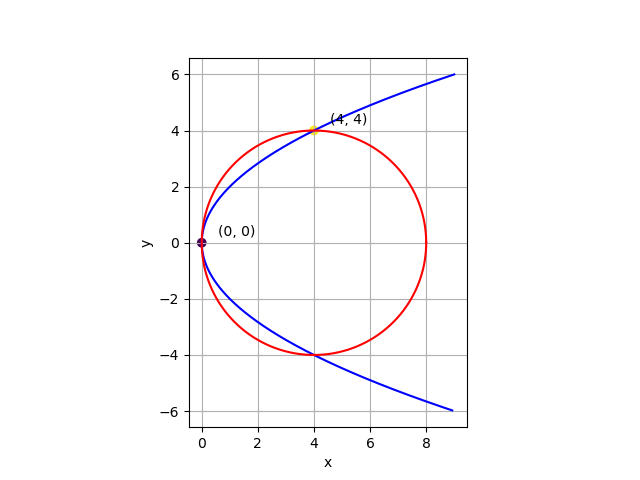
\includegraphics[width=0.7\linewidth]{/home/gvt/Documents/sdcard/github/EE1030/Assignment3/figs/fig1.png}
       \caption{Points of trisection of A and B.}
       \label{graph}
    \end{figure}
\end{document}  
